\subsection{Qualitative Analysis of Attribution:}
\label{sec:sysml:casestudy:qualitative}
%The datasets consist of a varying distribution of episodes per author as well as variance in the ability to characterize of each author from their style. 
%For the remainder of 
In this section, we consider the average (euclidean) distance between each pair of episodes by the same author as a heuristic for stylometric identifiability (SI), where lower average distance corresponds to higher SI and vice versa. 
Somewhat surprisingly, 
%we found that the number of episodes for each author is not correlated with the stylometric identifiability (SI). 
authors with a small number of total episodes ($<10$) were found at both extremes of identifiability, while the authors with the highest number of episodes were in the intermediate regions, suggesting that SI is not strongly correlated with episode length.  Next, we further investigate these groups.
%We next drill down on this further.
%In this subsection, we supplement the aforementioned metric-based comparisons from \S\ref{sec:analysis} with a qualitative characterization of these extremes.

\noindent \textbf{High SI authors:} 
Among the 20 users with the lowest average distance between episodes, a single pattern is prominent. 
This first group of high SI users are "newbie" users.  On a majority of analyzed forums, a minimum number of posts by a user is required before posting restrictions are removed from the user's account.
Thus, users create threads on `Newbie Discussion' subforums.
Typical posts on these threads include repeated posting of the same message or numbered posts counting up to the minimum required. 
As users tend to make all these posts within a fixed time frame, the combination of repeated, similar stylistic text and time makes the posts easy to identify. 
Exemplar episodes from this "newbie" group are shown in Table~\ref{tab:example_posts}. 
%Note that the writing style of an author may not be captured by such posts, but there exist accounts with posts only in these threads, therefore there is no other way to characterize these users. 

After filtering these users out, we identified a few more notable high SI users.
These include an author on BMR with frequent `\pounds' symbol and ellipses (`...') and an author on Agora who only posted referral links (with an eponymous username `ReferralLink'). 
Finally, restricting posts to those made by 200 most frequently posting users (henceforth, T200), we found a user (labeled HSI-Sec\footnote{pseudonym}) who frequently provided information on security, where character n-grams corresponding to `PGP', 'Key', 'security' are frequent (Table~\ref{tab:attribution}). 
Thus, \SYSMLmethodname{} is able to leverage vocabulary and punctuation-based cues for SI.

\noindent \textbf{Low SI authors:}  Here, we attempt to characterize the post episode styles that are challenging for \SYSMLmethodname{} to attribute to the correct author.
Seminal work by~\citet{brennan2009practical, brennan2012adversarial} has demonstrated that obfuscation and imitation based strategies are effective against text stylometry.
We analyze the T200 authors who had high inter-episode distances to ascertain whether this holds true for \SYSMLmethodname{}.
For the least (and third least) identifiable author among T200, we find that frequent word n-grams are significantly less frequent than those for the most identifiable author from this subset (most frequent token occurs $\sim 600$ times vs. $\sim 4800$ times for identifiable) despite having more episodes overall. 
Further, one of the most frequent tokens is the \texttt{{[QUOTE]}} token, implying that this author frequently incorporates other authors' quotes into their posts.  
This strategy is analogous to the imitation based attack strategy proposed by~\citet{brennan2012adversarial}.
%Similar observations hold for the third-least identifiable author in T200.
For the second least identifiable T200 author, we find that the frequent tokens have even fewer occurrences, and the special token \texttt{{[IMAGE]}} and its alternatives are among the frequent tokens - suggesting that an obfuscation strategy based on diversifying the vocabulary is effective.
Some samples are presented in Table~\ref{tab:attribution} under LSI-1 and LSI-2.
%This observation of low SI is maintained for the diversity in subforums posted on as well. 

\begin{table}
    \centering
    \begin{tabularx}{\linewidth}{XX}
    \toprule
        Thread & Posts  \\
    \midrule
         Spam to 50 \&  Get out of Noobville &  26, 27, 28, 29, 30 \\
         %\hline
         Post 30 Times $\dots$ To Post Anywhere& 7, 8, 9, $\dots$\\ 
         %\hline
         Spam to 50 $\dots$ & 46, 47, $\dots$, Yeah 50 Spam! \\
         %\hline
         $\dots$ use my link $\dots$ & {[LINK]}, Here is my ref link {[LINK]}, Try this link {[LINK]}, $\dots$\\
    \bottomrule
    \end{tabularx}
    \caption{Examples of highly identifiable posts.}
    \label{tab:example_posts}
\end{table}
\newcolumntype{s}{>{\hsize=.1\hsize}X}
\begin{table}
\begin{tabularx}{\linewidth}{sX}
\toprule
Author & Word Importance \\
\midrule
 & $\dots$ 2 cents, anyway $\dots$ 
PGP Key\colorbox[rgb]{0.8424999999999999, 0.9775000000000001, 0.8424999999999999}{ Fingerprint} = $\dots$\\
HSI-Sec & $\dots$ 
PGP Key\colorbox[rgb]{0.9124999999999999, 0.9875, 0.9124999999999999}{ Fingerprint} $\dots$ \colorbox[rgb]{0.8600000000000002, 0.9799999999999999, 0.8600000000000002}{...} $\dots$ security is NOT\colorbox[rgb]{0.8074999999999999, 0.9725000000000001, 0.8074999999999999}{ retroactive}. 
\\
& $\dots$ Is it possible for a\colorbox[rgb]{0.8775, 0.9825000000000002, 0.8775}{ gpg}\colorbox[rgb]{0.9475, 0.9924999999999999, 0.9475}{ key}\colorbox[rgb]{0.9924999999999999, 0.9475, 0.9475}{ to} request that ) \\
\hline
 & Check out the\colorbox[rgb]{0.985, 0.8949999999999999, 0.8949999999999999}{ link} in my sig $\dots$ \colorbox[rgb]{0.9475, 0.9924999999999999, 0.9475}{ [}\colorbox[rgb]{0.9475, 0.9924999999999999, 0.9475}{IMAGE} alt=8)]\\
LSI-1 & Hey dude, just run a search $\dots$\colorbox[rgb]{0.9875, 0.9124999999999999, 0.9124999999999999}{ I} can not help much $\dots$ \colorbox[rgb]{0.9875, 0.9124999999999999, 0.9124999999999999}{ Im} sure if you ask $\dots$ German\colorbox[rgb]{0.9475, 0.9924999999999999, 0.9475}{,} he may be willing to lend a hand. Good luck freind\colorbox[rgb]{0.7024999999999998, 0.9575000000000001, 0.7024999999999998}{ [}\colorbox[rgb]{0.4049999999999999, 0.9150000000000001, 0.4049999999999999}{IMAGE} alt=8)]\\
\midrule 
& [\colorbox[rgb]{0.9924999999999999, 0.9475, 0.9475}{QUOTE}] From: $\dots$ Just my opinion,\colorbox[rgb]{0.9124999999999999, 0.9875, 0.9124999999999999}{ I}\colorbox[rgb]{0.8949999999999999, 0.985, 0.8949999999999999}{'ve} done just about everything, $\dots$ \colorbox[rgb]{0.7900000000000001, 0.9699999999999999, 0.7900000000000001}{IMAGE} alt=8)] couldnt agree more\\
LSI-2 & [\colorbox[rgb]{0.9299999999999999, 0.99, 0.9299999999999999}{QUOTE}]\colorbox[rgb]{0.8250000000000002, 0.9749999999999999, 0.8250000000000002}{ From}\colorbox[rgb]{0.8775, 0.9825000000000002, 0.8775}{:} $\dots$  \colorbox[rgb]{0.9475, 0.9924999999999999, 0.9475}{ strangely} enough, when im in $\dots$ I too jabber\colorbox[rgb]{0.985, 0.8949999999999999, 0.8949999999999999}{ meaningless} jibberish $\dots$ \\
\bottomrule 
&Negative \fcolorbox{black}[rgb]{0.9000000000000001, 0.2999999999999998, 0.2999999999999998}{\rule{0pt}{2pt}\rule{2pt}{0pt}} Neutral \fcolorbox{black}[rgb]{1.0, 1.0, 1.0}{\rule{0pt}{2pt}\rule{2pt}{0pt}} Positive \fcolorbox{black}[rgb]{0.125, 0.875, 0.125}{\rule{0pt}{2pt}\rule{2pt}{0pt}}
\end{tabularx}

\caption{Integrated Gradient based attribution of posts}
\label{tab:attribution}
\end{table}

% A majority of this table is auto-generated. Please modify carefully
%\subsection{Gradient-based attribution}
\noindent \textbf{Gradient-based attribution:} To cement our preceding hypotheses, 
%we investigated whether neural network attribution methods support the qualitative observations from the previous section. Specifically, 
we investigate whether the generated embedding can be attributed to phrases in the input which were mentioned in the previous section. 
We use Integrated Gradients~\cite{sundararajan2017axiomatic}, an axiomatic approach to input attribution.
Integrated Gradients assign an importance score to each feature which corresponds to an approximation of the integral of the gradient of a model's output with respect to the input features along a path from some reference baseline value (in our case, all \texttt{[PAD]} tokens) to the  input feature.
%We used an implementation from the Captum python library~\cite{kokhlikyan2020captum} that uses the Gauss-Legendre quadrature rule for approximating the gradient.
In Table~\ref{tab:attribution}, the highlight color corresponds to the attribution importance score for the presented posts.
We observed that the attribution scores correspond to our intuitions: HSI-Sec had high importance for security words, LSI-1 had obfuscated posts due to the presence of common image tokens, and LSI-2 had quotes mixed in, lead to misattribution (imitation-like strategy).
%These observations provided further support to our preceding hypothesis about SI.


\begin{figure}
    \centering
    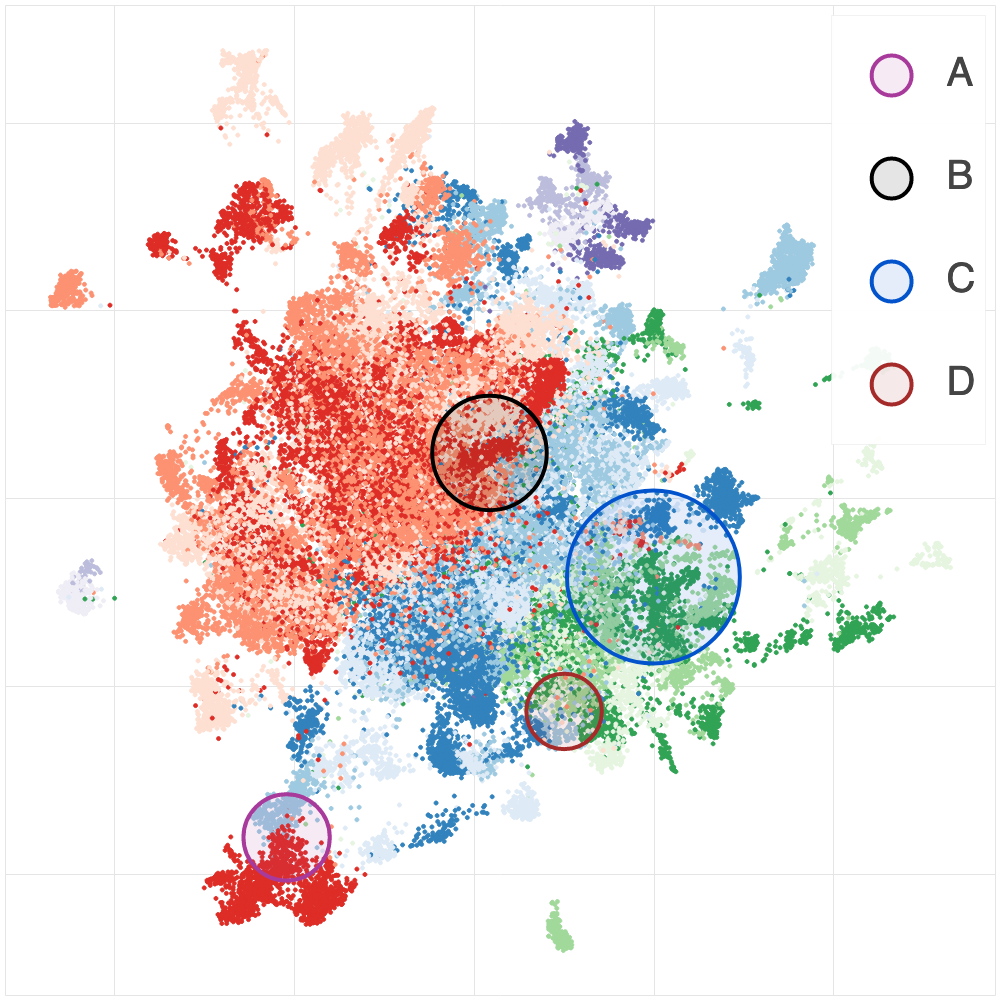
\includegraphics[width=\linewidth]{sysml/plots/cross_study.png}
    \caption{UMAP visualization of cross dataset embeddings for the top 200 authors, one hue per market. Circles denote the same user in two different markets. 
    %Each circle covers a large percentage of a users' posts over two markets
    }
    \label{fig:cross_dataset}
\end{figure}


%\noindent {\bf Migrant Analysis}
\subsection{Migrant Analysis}
%Cross-market alignment is achieved using a small sample of users matched by a high-precision heuristic (PGP key match). 
%Other heuristics (eg. shared username) can also be used as indicators of an author migrating between two markets.
To understand the quality of alignment from the episode embeddings generated by our method, we use a simple top-k heuristic: for each episode of a user, find the top-k nearest neighboring episodes from other markets, and count the most frequently occurring user among these (candidate sybil account).
Figure~\ref{fig:cross_dataset} shows a UMAP projection for T200. 
Users of each market are colored by sequential values of a single hue (i.e., reds - SR2, blues - SR, etc.).
%We select pairs of users such that for each pair $(u, v)$, $u$ is the most frequent neighbor of $v$, and $v$ is the most frequent of $u$ in the top-k neighbors ($k = 10$).
The circles in the figure highlight the top four pairs of users (top candidate sybils) with a frequent near neighbor from a different market. 
We find that each of these pairs can be verified as sybil accounts, either by a shared username (A, C, D) or by manual inspection of posted information (B).   
Note that none of these pairs were pre-matched using PGP - none were present in the high-precision matches. Thus,
\SYSMLmethodname{} is able to identify high ranking sybil matches reflecting users that migrate from one market to another.

\pmcomment{TODO: Add additional results from Darkweb folder discussion.}